\section{Gateway Protocol Solution Overview}\label{sec:solution}
The Gateway Protocol is a cross-chain oracle token model that enables any application operating on a decentralized ledger (i.e., a dApp) to add a permissioning layer that adheres to predetermined requirements. The protocol allows dApps to meet AML/KYC requirements of an industry or location without developing their own systems for identity verification or secure data storage.

Identity verification is completed by one or more Gatekeepers belonging to a Gatekeeper network. Each Gatekeeper network will enforce a specific set of requirements, which may be modeled on a set of trading regulations, e.g., those active in a DEX user’s country of residence. Requirements may include age, country of residence, IP address, investor status, and more. Once a Gatekeeper has verified an individual’s identity and conformance with the requirements, it will issue them with a Gateway Pass.

To take part in the ecosystem, a dApp simply extends its existing interfaces to require the presence of a specific and active Gateway Pass within an individual’s wallet. If the appropriate Pass is present and active, the individual can interact with the dApp as usual. If a Pass isn’t present, the individual is first directed to an appropriate Gatekeeper network to undergo the verification process.

The Gatekeeper Protocol is managed by a Decentralized Autonomous Organization (DAO), which decides on the evolution of the protocol. The DAO is involved in operational decisions like the appointment of Guardians and maintenance of Gatekeeper network processes. The DAO operates via a voting system, allowing Governance Token holders to propose and vote on changes to the Ecosystem.

Gateway Protocol contracts can be deployed on any compatible chain, allowing integration on a wide range of Blockchains and Applications.

\subsection{Personas in the Gateway Pass Ecosystem}

There are three primary personas within the ecosystem: \textbf{dApps}, \textbf{Gatekeepers}, and \textbf{Gateway Pass Users}. These personas will play a direct role in issuing, using, and verifying Gateway Passes.

Two further personas play a supporting role: \textbf{Gateway Pass Holders} and \textbf{Guardians}. These personas will enable the operations and continued maintenance of individual Gatekeeper networks through voting, admitting new gatekeepers, etc.

\subsubsection{dApps (Gateway Pass Verifiers)}
dApps are the primary beneficiaries of the Gateway Protocol. It enables a dApp to adhere to any set of KYC/AML requirements without developing its own verification process. Instead, a dApp verifies the presence and validity of a relevant Gateway Pass before allowing a User to access the service.

\begin{figure}[h]
  \begin{center}
    \centering
    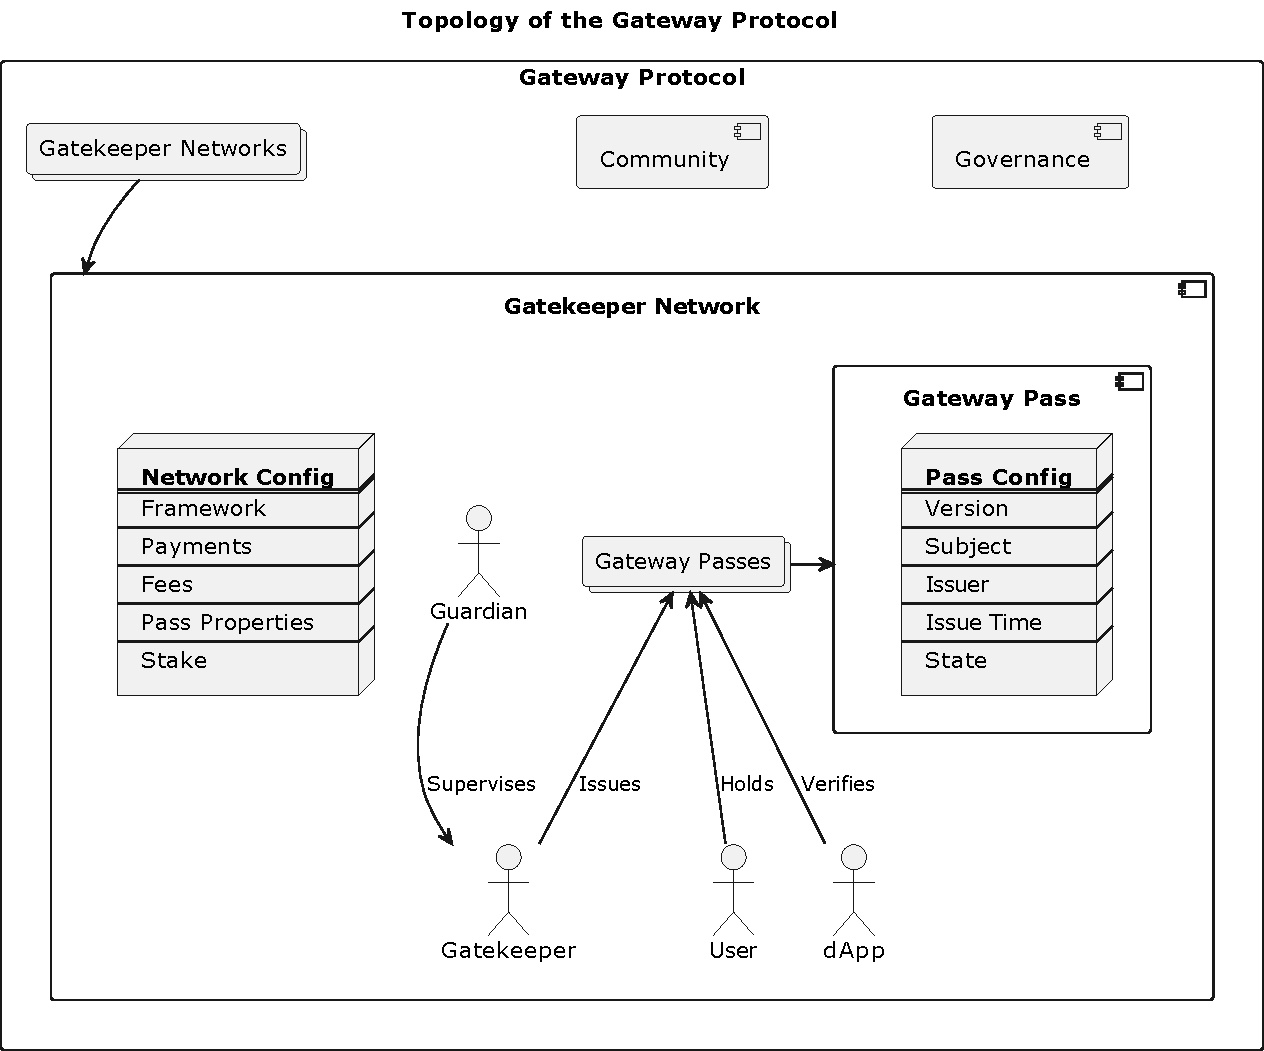
\includegraphics[width=0.8\textwidth]{figures/02-solution-topology.pdf}
    \caption[Fig 3]{Topology and components of the Gateway Protocol}
  \end{center}
\end{figure}

To take part, a dApp integrates with one or more Gatekeeper networks and establishes a Custodial Wallet from which Gatekeepers can draw any funds they are owed for using verified Gateway Passes by that Gatekeeper. This process will be explained in more detail in the ‘Gatekeeper Incentives’ section.

\vspace{1em}

\textbf{Motivation:}
\begin{itemize}
\item Easily adhere to any set of legal, regulartory or technical requirements.
\item Externalize the verification and enforcement of framework rules to the Gatekeeper network
\end{itemize}

\textbf{Role in the Ecosystem:}
\begin{itemize}
\item Funds the verification process through payments to Gatekeepers. This cost can be offset to Users of the dApp.
\item May also participate in Protocol governance by staking as a Governance Token Holder.
\end{itemize}

\subsubsection{Gatekeepers (Gateway Pass Issuers)}
A Gatekeeper is any legal entity that can fulfill the requirements of a Gatekeeper network. Each Gatekeeper's ability to do so is verified and audited by the Guardian on an ongoing basis.

Gatekeepers are the service providers of the Gateway Protocol. Each Gatekeeper belongs to one or more Gatekeeper networks and is responsible for enforcing the requirements of those networks by verifying users per those requirements—for example, by verifying a User’s age and location.

Gatekeepers are also involved in the governance of Gatekeeper networks and have a vested interest in maintaining each network’s requirements in line with any relevant regulations or frameworks.

\vspace{1em}

\textbf{Motivation:}
\begin{itemize}
\item Gatekeepers are compensated for Verification Services or Gateway Pass utilization in governance tokens.
\end{itemize}

\textbf{Role in the Ecosystem:}
\begin{itemize}
\item Completes the User verification process.
\item Issues, Freezes, and Revokes Gateway Pass in accordance with a User’s compliance (or lack of compliance) with a Gatekeeper network’s requirements.
\end{itemize}

\subsubsection{Gateway Pass Users}
Gateway Pass Users are individuals who wish to interact with a dApp that is part of the Gateway Pass ecosystem.

\vspace{1em}

\textbf{Motivation:}
\begin{itemize}
\item Users must acquire a Gateway Pass from a relevant Gatekeeper network before accessing services offered by participating dApps.
\item Evidence provided to a Gatekeeper by the User is protected and remains private and apart from a pseudonymous Gateway Pass, no personal information is put in the public space.
\end{itemize}

\textbf{Role in the Ecosystem:}
\begin{itemize}
\item Must approach a Gatekeeper from a relevant Gatekeeper network and provide requested evidence to satisfy the network’s requirements.
\end{itemize}

\subsubsection{Voters (Governance Token Holders)}
Voters maintain the DAO Ecosystem by proposing and voting on changes. Any individual or organization that holds Gateway Passes has the right to vote on proposals. Staking will be required to propose a change to the DAO Ecosystem.

Gatekeepers will usually also be voters, as they have a vested interest in protecting, updating, and introducing requirements. Guardian Governance may transition to voters to further decentralize the Ecosystem in the future.

\vspace{1em}

\textbf{Motivation:}\\
Any party with an interest in the Gateway Protocol and/or DAO Ecosystem has a vested interest in ensuring its continued operation and effectiveness. Holding Governance Tokens provides parties with the opportunity to influence these operations.

\vspace{1em}

\textbf{Role in the Ecosystem:}\\
Proposing and voting on changes, such as:
\begin{itemize}
\item Proposing a new Gatekeeper network with predefined requirements.
\item Changing the requirements of an existing Gatekeeper network.
\item Supporting Governance Token utilization.
\end{itemize}

\subsubsection{Guardian}
The Guardian supervises the ecosystem and protocol and ensures each Gatekeeper network correctly adheres to its requirements.

\vspace{1em}

\textbf{Motivation:}
\begin{itemize}
\item Are experts in a specific regulatory or legal framework and want to enable compliance in a web3-context.
\item Fee-based income model through network operations and Gatekeeper staking.
\end{itemize}

\textbf{Role in the Ecosystem:}
\begin{itemize}
\item Regularly audits Gatekeepers on their off-chain verification and evidence data.
\item Slashes Governance Token stake for Gatekeepers that fail to meet requirements.
\item Removes Gatekeepers that continually fail to meet requirements or act maliciously.
\item Audits and accepts new Gatekeepers into Gatekeeper networks.
% \item Maintains on-chain smart contracts for the Gateway Protocol.
\item Supports Governance Token utilization.
\end{itemize}

\subsection{What is a Gatekeeper Network Framework?}
A Gatekeeper network framework is the set of requirements a User must meet to obtain a Gateway Pass from a Gatekeeper. Similarly, the framework is also the set of requirements a Gatekeeper must enforce before issuing a Gateway Pass.

Each framework will have its own Gatekeeper network, and each Gatekeeper network will only enforce one framework. However, a Gatekeeper can be part of as many Gatekeeper networks as desired, so long as it is competent to enforce the associated framework and prove that to the Guardian.

\subsection{End User Experience}
Users that already have a relevant Gateway Pass in their wallet can interact seamlessly with participating dApps with no additional steps. Users that don’t already have a relevant Pass will be directed to the appropriate Gatekeeper network—ideally providing them with several Gatekeepers to choose from—where they will undergo the verifications needed to issue a Pass.

The verification process will vary depending on the framework of the relevant Gatekeeper network. For example, some dApps may require users to undergo a stringent identity verification process, while others may simply need proof that the User is over a certain age.\\
